\section{Introduction}\label{sec:intro}

A central goal of machine learning research is to develop a universal architecture capable of learning and reasoning across a wide range of tasks and data modalities. Theoretical frameworks for understanding human and animal intelligence seek to explain intelligent behavior through a small set of fundamental principles~\citep{marcus2003algebraic}. However, in machine intelligence, there is a tension between the objective of developing a \textit{general} architecture and the need to incorporate \textit{inductive biases} that are beneficial for specific tasks~\citep{wolpert1995no,baxter2000model}. When faced with finite training data and numerous solutions to empirical risk minimization, inductive biases steer the learning algorithm towards solutions with desirable properties, enhancing data efficiency and generalization.
A core scientific challenge of machine learning is to identify a complete and broadly applicable set of inductive biases that promote robust, flexible, and data-efficient learning across a diverse set of problems.
% There is, however, a tension between the goal of creating a general architecture and the need to incorporate inductive biases that are beneficial for specific tasks~\citep{wolpert1995no,baxter2000model}.
% In machine intelligence, the scientific challenge is to identify a complete set of fundamental inductive biases with broad applicability to real-world problems that enable robust, flexible, and data-efficient learning.

Relational reasoning is a central component of generally intelligent systems and is believed to underlie human abilities for abstraction and systematic generalization~\citep{gentner1983structure,snow1984topography,kemp2008discovery,holyoak2012analogy}. The power of relational reasoning lies in its capacity to generate inferences and generalizations in systematic and novel ways, even across instances which are superficially very different but have similarities on an abstract structural level. This grants humans a capacity for out-of-distribution generalization, data efficiency, and continual learning, which modern machine learning is yet to match~\citep{lake2017building,smith2019promise,nogueira2021investigatinglimitationstransformerssimple}. Replicating this ability in machine intelligence can ultimately lead to universal inductive generalization from a finite set of observations to an infinite set of novel instances~\citep{goyal2022inductive}.

The ability of artificial intelligence systems to perform relational reasoning has long been an area of active study across various approaches to AI. In symbolic modeling frameworks, the relationships between symbols are explicitly defined in the language of logic and mathematics~\citep{newell1980physical,harnad1990symbol,fodor1988connectionism}. However, such approaches often require hand-crafted representations and suffer from the symbol grounding problem, limiting their ability to generalize to variations in the task or input outside a certain domain. By contrast, deep learning approaches build data-dependent representations that are, in principle, capable of generalizing across diverse conditions. However, recent work exploring the ability of deep learning models to learn relational tasks finds that seemingly simple relational inferences can be remarkably difficult for powerful neural network architectures~\citep{lake2018generalization,barrett2018measuring,hill2018learning,webbEmergentSymbolsBinding2021,santoroSimpleNeuralNetwork2017,shanahanExplicitlyRelationalNeurala,kergNeuralArchitectureInductive2022,altabaa2024abstractors,altabaaLearningHierarchicalRelational2024}. An emerging hypothesis, which we explore further here, explains this through the lens of inductive biases, arguing that neural networks struggle with relational reasoning because they overemphasize individual object representations---\textit{sensory} information---while lacking \textit{explicit} mechanisms for encoding and processing \textit{relational information}~\citep{webbRelationalBottleneckInductive2024}.

In this work, we explore this idea in the context of the Transformer architecture~\citep{vaswani2017attention}, which offers a promising starting point for building a versatile, general-purpose neural architecture. Although Transformers, like other neural architectures, struggle to learn abstract relational representations~\citep{santoroSimpleNeuralNetwork2017,shanahanExplicitlyRelationalNeurala,kergNeuralArchitectureInductive2022,altabaa2024abstractors,altabaaLearningHierarchicalRelational2024}, there is encouraging evidence that Transformer-based foundation models acquire some relational reasoning ability~\citep{wei2022chain,kojima2022large,valmeekam2022large,huang2023reasoninglargelanguagemodels,webb2023emergent,huang2024largelanguagemodelsselfcorrect,mirzadeh2024gsmsymbolicunderstandinglimitationsmathematical} through large-scale training on large amounts of data~\citep{brown2020languagemodelsfewshotlearners,kaplan2020scalinglawsneurallanguage,hoffmann2022trainingcomputeoptimallargelanguage,grattafiori2024llama3herdmodels}. This presents an opportunity to explore Transformer-based architectures with built-in neural mechanisms and inductive biases for explicit and enhanced relational reasoning capabilities, seeking to imbue the Transformer architecture with a greater capacity for efficient induction of abstractions.

To introduce our proposal, we highlight a distinction between two types of information which are encoded in the internal representation of Transformer models: \textit{sensory information}, which represents features of individual objects, and \textit{relational information}, representing comparisons and relationships between objects. In the standard attention mechanism of Transformers, relational information is \textit{entangled} with sensory information, limiting the model's ability to learn to explicitly represent and reason about the relationships between objects. In particular, in standard attention, relational information \textit{directs} the flow of information (i.e., attention scores encoding a selection criterion), while the \textit{values} routed are representations of the sensory attributes of individual objects. In this work, we explore a new type of attention mechanism we call \textit{relational attention}, in which the values being routed are themselves representations of relationships between the source and the target, computed explicitly as a series of comparisons under learned feature maps. This equips the model with a mechanism for explicitly routing and processing relational information, decoupling it from sensory features.

We integrate relational attention with the standard attention mechanism of Transformers, yielding a variant of multi-head attention that processes both sensory and relational information in parallel. The resulting \textit{Dual Attention Transformer (DAT)} architecture disentangles the two types of information during the information retrieval stage and integrates them during the local processing stage of each layer. We empirically evaluate this architecture on a diverse set of tasks, ranging from synthetic benchmarks on relational reasoning to complex real-world tasks such as language modeling and visual processing. Our results demonstrate that integrating explicit relational mechanisms into the Transformer architecture leads to significant performance gains in terms of data efficiency and parameter efficiency.

\begin{figure*}
  \centering
  \begin{subfigure}[t]{0.415384615\textwidth} % 0.9 * 3 / 6.5
    \centering
    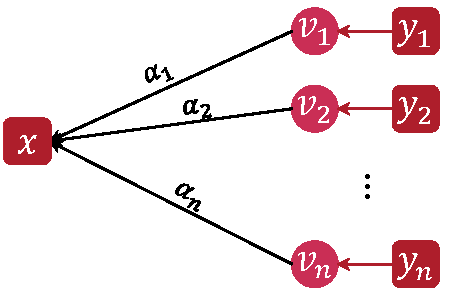
\includegraphics[width=0.8\textwidth]{figs/sensory_retrieval.pdf} % size: 3 x 2 in
    \caption{$\Attn(x, \ys)$}%: Retrieval of sensory information by standard attention.}
  \end{subfigure}
  \qquad
  \begin{subfigure}[t]{0.484615385\textwidth} % 0.9 * 3.5 / 6.5
    \centering
    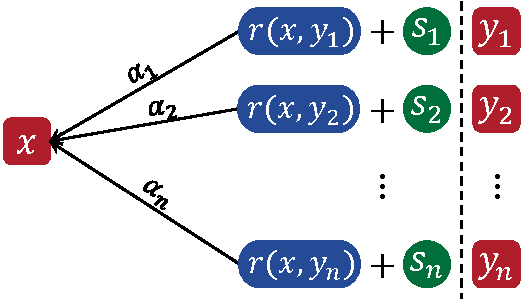
\includegraphics[width=0.8\textwidth]{figs/relational_retrieval.pdf} % size 3.5 x 2 in
    \caption{$\RelAttn(x, \ys)$}%: Retrieval of relational information by relational attention.}
  \end{subfigure}
  % 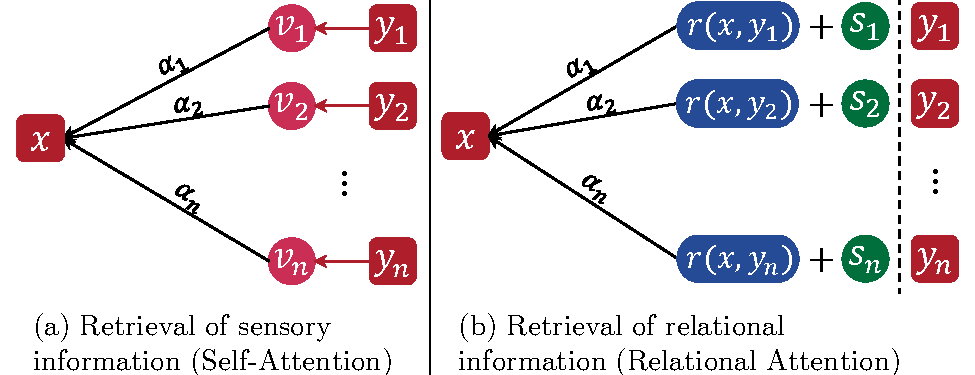
\includegraphics[width=0.8\textwidth]{figs/attn_fig_combined_noqeuerykey.pdf}
  \caption{Standard self-attention retrieves sensory information $v_i$ about the attributes of individual objects while relational attention retrieves relational information $r(x, y_i)$ about the relationship between the objects in the context and the target.
  Each relation is tagged with a symbol $s_i$ which acts as an abstract variable identifying the source.
  In both cases, information is aggregated according to the attention scores $\alpha_i$, which are computed by a softmax over inner products of queries and keys.
  }\label{fig:selfattn_relattn}
  % \vskip-12pt
\end{figure*}
